% !TEX program = xelatex

\documentclass[12pt,a4paper]{article}
\usepackage[UTF8]{ctex}
\usepackage{float}
\usepackage{amsmath}
\usepackage{amsfonts}
\usepackage{enumerate}
\usepackage{booktabs}
\usepackage{graphicx}
\usepackage{longtable}
\usepackage{subfigure}
\usepackage{multirow}
\usepackage{url}

% for plotting 
\usepackage{caption}
\usepackage{pgfplots}

% for pseudo code 
\usepackage{algorithm}
\usepackage[noend]{algpseudocode}

% for reference 
\usepackage{hyperref}
\usepackage{cleveref}
\crefname{equation}{方程}{方程}
\Crefname{equation}{方程}{方程}
\crefname{table}{表}{表}
\Crefname{table}{表}{表}
\crefname{figure}{图}{图}
\Crefname{figure}{图}{图}

% for code 
\usepackage{listings}
\usepackage{xcolor}
\usepackage{fontspec}
\definecolor{darkgreen}{rgb}{0,0.6,0}
\newfontfamily\consolas{Consolas}

\lstset {
    basicstyle=\footnotesize\consolas, % basic font setting
    breaklines=true, 
    frame=single,     % {single, shadowbox, bottomline}
    keywordstyle=\color{blue}, 
    commentstyle=\color{darkgreen},
    stringstyle=\color{red},
    showstringspaces=false,
    % backgroundcolor=\color{black!5}, % set backgroundcolor
    % numbers=left, 
    % numberstyle=\consolas,
}

% Microsoft Word A4 paper default layout 
\usepackage[a4paper, left=3.18cm, right=3.18cm, top=2.54cm, bottom=2.54cm]{geometry}

\captionsetup[figure]{labelfont={bf}, name={图}}
\captionsetup[table]{labelfont={bf}, name={表}}

\title{DIP: Project 1}
\author{2017011620 \quad 计73 \quad 李家昊}
\date{\today}

\begin{document}

\maketitle

\section{Image Fusion}

\subsection{方法}

根据Poisson Image Processing~\cite{perez2003poisson}中的Guided Interpolation方法,记插值区域为$\Omega$,目标图像的颜色函数为$f^*$,插值后$\Omega$区域内颜色函数为$f$,由于可以对RGB三通道分别处理,因此颜色可视作标量,现给定一个参考梯度场$\mathbf{v}$,希望插值后$\Omega$区域内的梯度与参考梯度尽可能一致,且满足$\Omega$的边界值与目标图像相同,这样就得到一个带有Dirichlet边界条件的扩展Laplace方程,
\begin{equation}\label{eq:continuous}
    \min_{f} \iint_\Omega | \nabla f - \mathbf{v}|^2 \text{ with } f|_{\partial \Omega} = f^*|_{\partial \Omega}
\end{equation}

\Cref{eq:continuous}可离散化如下,
\begin{equation}\label{eq:discrete}
    \forall p \in \Omega, \quad |N_p|f_p - \sum_{q\in N_p \cap \Omega} f_q = \sum_{q \in N_p \cap \partial \Omega} f_q^* + \sum_{q\in N_p} v_{pq}
\end{equation}

其中,对于$\Omega$区域内的一个像素位置$p$,$N_p$为$p$的邻居集合,包含上下左右四个方向,对于$p$的某个邻居$q \in N_p$,$v_{pq}$为从$p$到$q$的参考梯度。

对于Image Fusion来说,可以采用Seamless Cloning的方法,将原图的梯度场作为参考梯度场。记原图的颜色函数为$g$,则有$\mathrm{v} = \nabla g$,因此$v_{pq} = g_p - g_q$,代入\Cref{eq:discrete}求解即可。

\subsection{实现细节}

在具体求解过程中,注意到\Cref{eq:discrete}是一个$|\Omega|$元线性方程组,可以将它记为$\mathbf{Ax} = \mathbf{b}$。其中,线性方程组的系数矩阵为$\mathbf{A}\in \mathbb{R}^{|\Omega|\times |\Omega|}$,对于$\forall p \in \Omega$,有$\mathbf{A}(p,p)=4$,且$\mathbf{A}(p,q)=-I_{q\in N_p\cap \Omega}$,其中$I$为示性函数。事实上,可以进一步观察到,矩阵$\mathbf{A}$的每一行最多只有5个元素,因此可采用稀疏矩阵的方式来存储。对于线性方程组的右端项$\mathbf{b}$,它的每一个分量$\mathbf{b}(p)$即为\Cref{eq:discrete}的右端。

得到系数矩阵$\mathbf{A}$和右端项$\mathbf{b}$后,可通过迭代方法求解线性方程组,得到的解$\mathbf{x}$即为融合后在$\Omega$区域内的颜色函数$f$。

\subsection{实验结果}

在给定的两组图片上,每组分别用无缝克隆的Poisson方法和直接裁剪拼接的Naive方法进行处理,生成的结果如\Cref{fig:result1}和\Cref{fig:result2}所示。可以看出,对于Poisson方法,图像边缘的过渡更加平滑和自然,同时保留了重要的原图信息。

\begin{figure}
    \centering
    \subfigure[Naive]{
        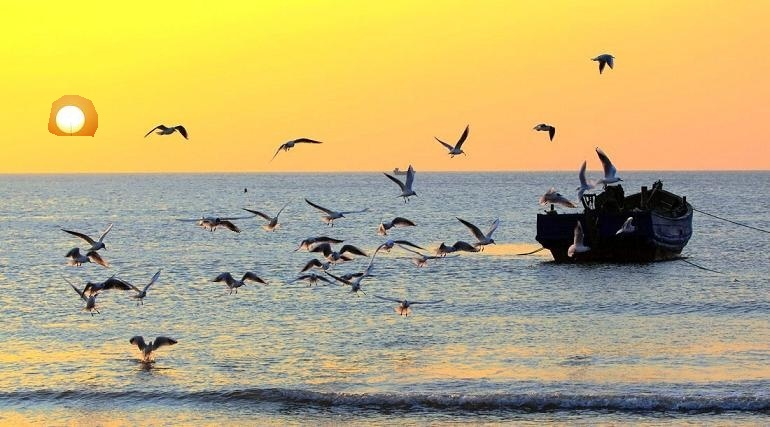
\includegraphics[width=0.47\textwidth]{../image_fusion/outputs/1/naive.jpg}
    }
    \subfigure[Poisson]{
        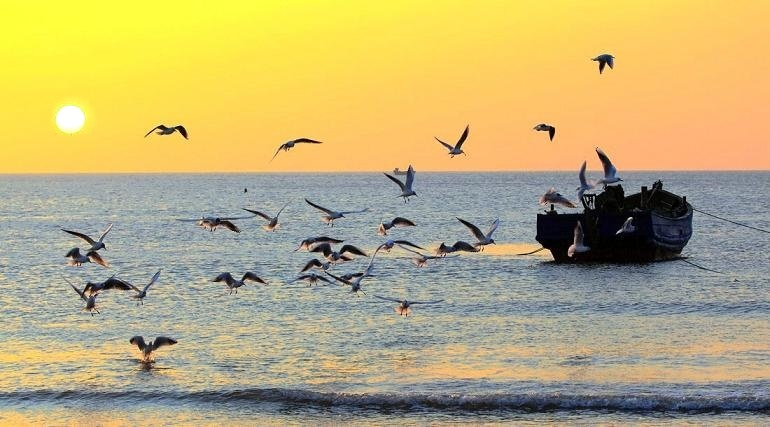
\includegraphics[width=0.47\textwidth]{../image_fusion/outputs/1/poisson.jpg}
    }
    \caption{第一组图片的融合效果}
    \label{fig:result1}
\end{figure}

\begin{figure}
    \centering
    \subfigure[Naive]{
        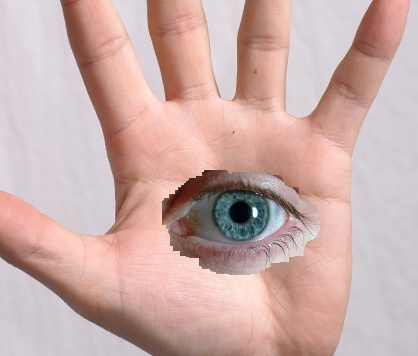
\includegraphics[width=0.47\textwidth]{../image_fusion/outputs/2/naive.jpg}
    }
    \subfigure[Poisson]{
        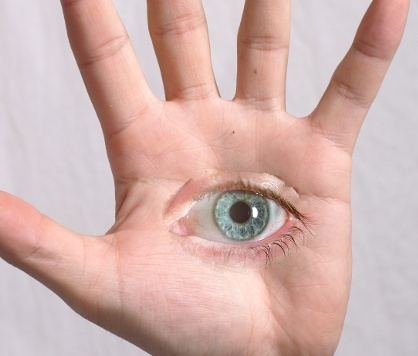
\includegraphics[width=0.47\textwidth]{../image_fusion/outputs/2/poisson.jpg}
    }
    \caption{第二组图片的融合效果}
    \label{fig:result2}
\end{figure}

\section{Face Morphing}

\subsection{方法}

在人脸融合任务中,需要根据原图和目标图求出中间状态。解决方法可大致分为形状融合和颜色融合两个步骤,即首先将原图和目标图分别对齐到中间状态,再将它们的颜色融合,这样就得到了最终融合的图像。

首先定义融合率$\alpha \in (0, 1)$,表示将目标图的权重置为$\alpha$,原图的权重置为$1-\alpha$,将原图和目标图加权平均后就得到中间状态。

对于形状融合,在齐次坐标意义下,首先标记出原图和目标图中对应的特征点$\{\mathbf{p}_i\}_{i=1}^n$和$\{\mathbf{q}_i\}_{i=1}^n$,则中间状态的特征点$\{\mathbf{r}_i\}_{i=1}^n$可由原图和目标图的对应特征点加权平均得到,
\begin{equation}
    \mathbf{r}_i = (1 - \alpha) \mathbf{p}_i + \alpha \mathbf{q}_i, \quad i = 1,2,\cdots,n
\end{equation}

为了将原图对齐到中间状态,首先对中间状态的特征点$\{\mathbf{r}_i\}_{i=1}^n$进行Delaunay三角剖分,然后将原图对应的三角形区域仿射变换到中间状态的三角形区域。具体来说,假设$(\mathbf{p}_1, \mathbf{p}_2,\mathbf{p}_3)$为原图的一个Delaunay三角,它对应的中间状态为$(\mathbf{r}_1, \mathbf{r}_2,\mathbf{r}_3)$,则仿射变换矩阵$\mathbf{A}$满足,
\begin{equation}
    \mathbf{A} (\mathbf{p}_1, \mathbf{p}_2, \mathbf{p}_3) = (\mathbf{r}_1, \mathbf{r}_2,\mathbf{r}_3)
\end{equation}

由此可求出$\mathbf{A}^{-1}$。再根据仿射变换,对于中间状态三角内的每个像素坐标$\mathbf{p}$,可得到它在原图的像素坐标为$\mathbf{A}^{-1} \mathbf{p}$,若不为整数,进行插值即可。

遍历每个Delaunay三角,在每个三角中遍历每个像素,即可将原图变换到中间状态。用相同的方法将目标图变换到中间状态,这样就将原图和目标图分别对齐到了中间状态。

对于颜色融合,记对齐到中间状态的原图和目标图分别为$\mathbf{I}$和$\mathbf{J}$,用同样的加权平均方法对整张图片进行Cross Dissolve即可,
\begin{equation}
    \mathbf{M} = (1-\alpha)\mathbf{I} + \alpha \mathbf{J}
\end{equation}

这样就得到了最终融合的图像$\mathbf{M}$。

\subsection{实现细节}

本实验最大的工作量在于特征点的标注,这里采用机器和人工相结合的方式。其中第一组图片中采用了Face++的人脸检测API来标注人脸图像,然后进行了手工修正,并增加了对头顶,发际线,耳朵,衣领等特征点的标记,第二组图片中,由于Face++ API无法识别狮子的脸,因此只能全部手工标注。

此外,标注前首先需要统一原图和目标图的大小,仿射变换的插值采用双线性插值,Delaunay三角剖分使用\texttt{scipy}库的实现。

\subsection{实验结果}

在给定的两组图片上,标定的特征点及Delaunay三角剖分如\Cref{fig:morph_features1}和\Cref{fig:morph_features2}所示,每组图片生成8个中间状态,得到的序列如\Cref{fig:morph_result1}和\Cref{fig:morph_result2}所示。

两组图片中,除了第一组图片的领结处有少量artifact之外,其他位置的过渡均十分自然。

\begin{figure}
    \centering
    \subfigure[Source Points]{
        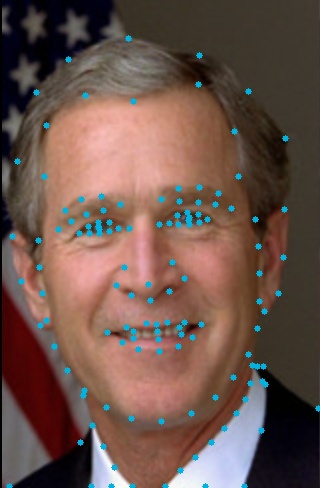
\includegraphics[width=0.20\textwidth]{../face_morphing/outputs/1/source_landmarks.jpg}
    }
    \subfigure[Source Delaunay]{
        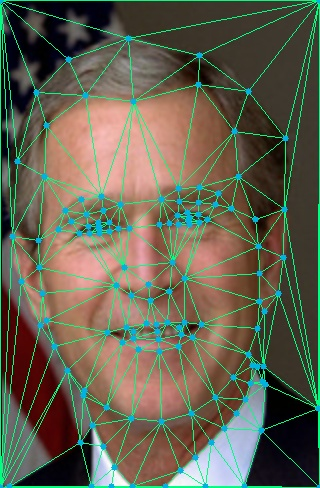
\includegraphics[width=0.20\textwidth]{../face_morphing/outputs/1/source_delaunay.jpg}
    }
    \subfigure[Target Points]{
        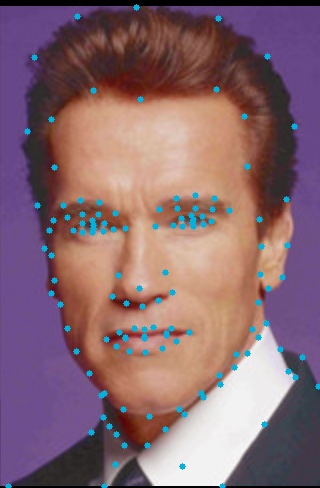
\includegraphics[width=0.20\textwidth]{../face_morphing/outputs/1/target_landmarks.jpg}
    }
    \subfigure[Target Delaunay]{
        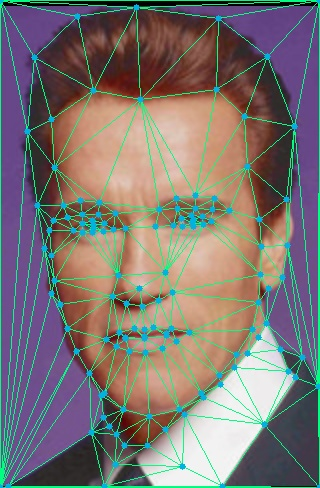
\includegraphics[width=0.20\textwidth]{../face_morphing/outputs/1/target_delaunay.jpg}
    }
    \caption{第一组图片的特征点及Delaunay三角剖分}
    \label{fig:morph_features1}
\end{figure}

\begin{figure}
    \centering
    \subfigure[Source]{
        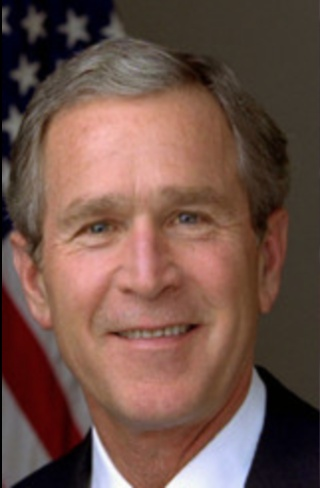
\includegraphics[width=0.17\textwidth]{../face_morphing/inputs/1/source.jpg}
    }
    \subfigure[$\alpha = 1/9$]{
        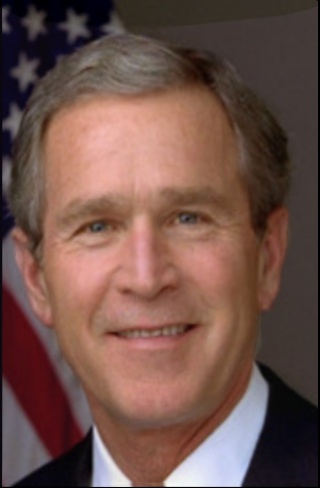
\includegraphics[width=0.17\textwidth]{../face_morphing/outputs/1/stage_1.jpg}
    }
    \subfigure[$\alpha = 2/9$]{
        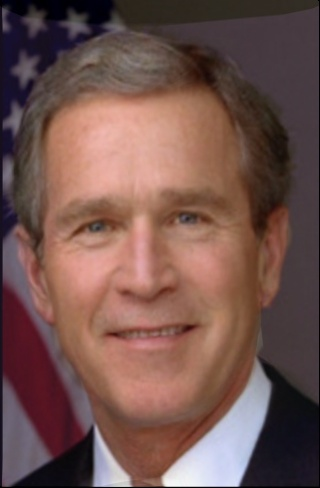
\includegraphics[width=0.17\textwidth]{../face_morphing/outputs/1/stage_2.jpg}
    }
    \subfigure[$\alpha = 3/9$]{
        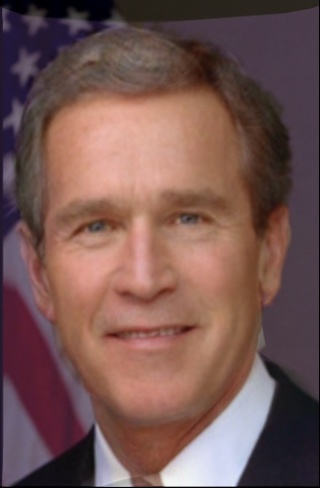
\includegraphics[width=0.17\textwidth]{../face_morphing/outputs/1/stage_3.jpg}
    }
    \subfigure[$\alpha = 4/9$]{
        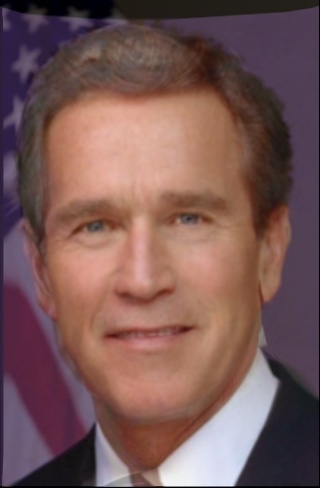
\includegraphics[width=0.17\textwidth]{../face_morphing/outputs/1/stage_4.jpg}
    }
    \subfigure[Target]{
        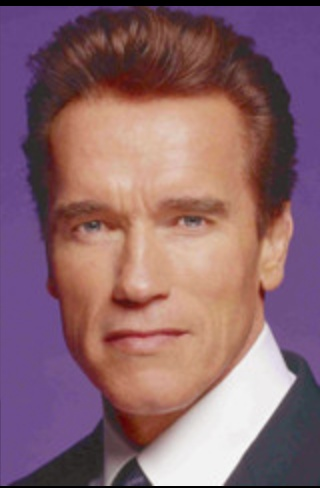
\includegraphics[width=0.17\textwidth]{../face_morphing/inputs/1/target.jpg}
    }
    \subfigure[$\alpha = 8/9$]{
        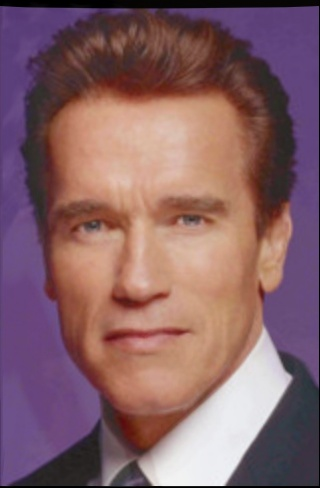
\includegraphics[width=0.17\textwidth]{../face_morphing/outputs/1/stage_8.jpg}
    }
    \subfigure[$\alpha = 7/9$]{
        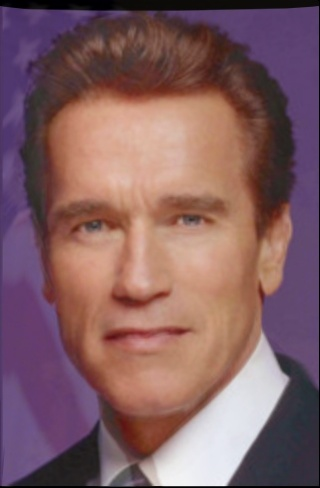
\includegraphics[width=0.17\textwidth]{../face_morphing/outputs/1/stage_7.jpg}
    }
    \subfigure[$\alpha = 6/9$]{
        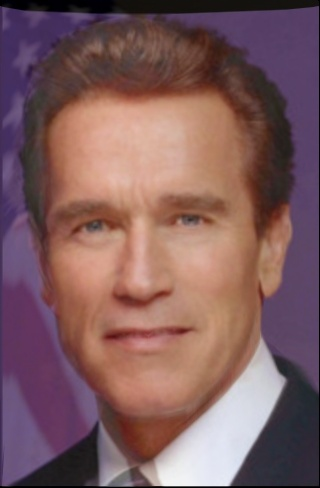
\includegraphics[width=0.17\textwidth]{../face_morphing/outputs/1/stage_6.jpg}
    }
    \subfigure[$\alpha = 5/9$]{
        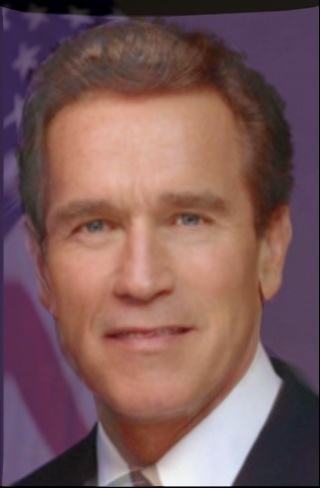
\includegraphics[width=0.17\textwidth]{../face_morphing/outputs/1/stage_5.jpg}
    }
    \caption{在不同的融合率$\alpha$下,第一组图片的融合效果}
    \label{fig:morph_result1}
\end{figure}

\begin{figure}
    \centering
    \subfigure[Source Points]{
        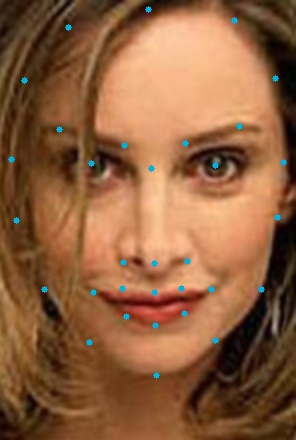
\includegraphics[width=0.20\textwidth]{../face_morphing/outputs/2/source_landmarks.jpg}
    }
    \subfigure[Source Delaunay]{
        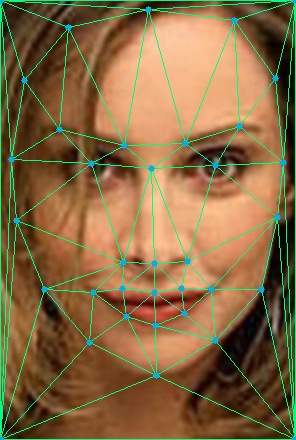
\includegraphics[width=0.20\textwidth]{../face_morphing/outputs/2/source_delaunay.jpg}
    }
    \subfigure[Target Points]{
        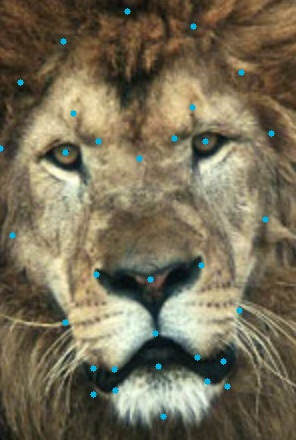
\includegraphics[width=0.20\textwidth]{../face_morphing/outputs/2/target_landmarks.jpg}
    }
    \subfigure[Target Delaunay]{
        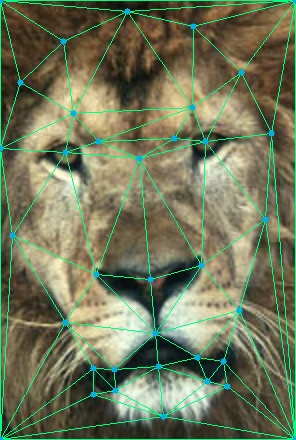
\includegraphics[width=0.20\textwidth]{../face_morphing/outputs/2/target_delaunay.jpg}
    }
    \caption{第二组图片的特征点及Delaunay三角剖分}
    \label{fig:morph_features2}
\end{figure}

\begin{figure}
    \centering
    \subfigure[Source]{
        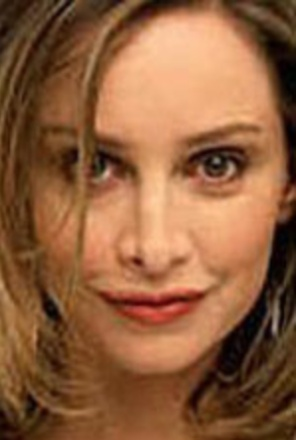
\includegraphics[width=0.17\textwidth]{../face_morphing/inputs/2/source.jpg}
    }
    \subfigure[$\alpha = 1/9$]{
        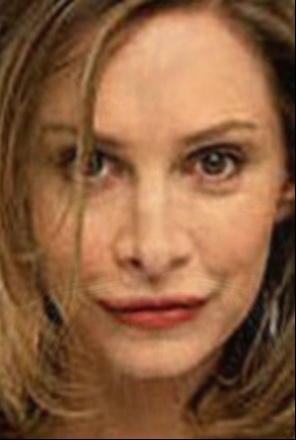
\includegraphics[width=0.17\textwidth]{../face_morphing/outputs/2/stage_1.jpg}
    }
    \subfigure[$\alpha = 2/9$]{
        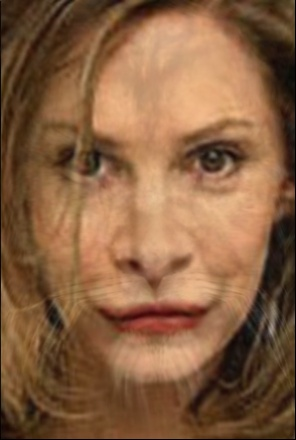
\includegraphics[width=0.17\textwidth]{../face_morphing/outputs/2/stage_2.jpg}
    }
    \subfigure[$\alpha = 3/9$]{
        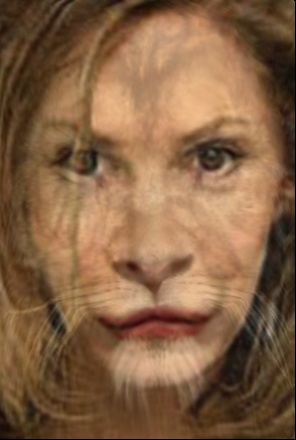
\includegraphics[width=0.17\textwidth]{../face_morphing/outputs/2/stage_3.jpg}
    }
    \subfigure[$\alpha = 4/9$]{
        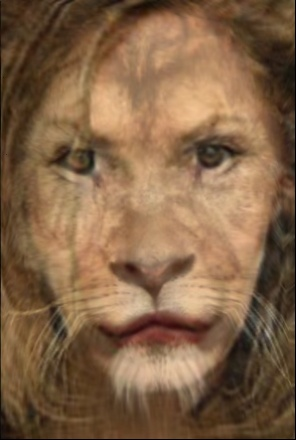
\includegraphics[width=0.17\textwidth]{../face_morphing/outputs/2/stage_4.jpg}
    }
    \subfigure[Target]{
        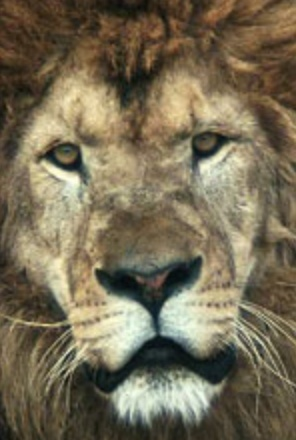
\includegraphics[width=0.17\textwidth]{../face_morphing/inputs/2/target.jpg}
    }
    \subfigure[$\alpha = 8/9$]{
        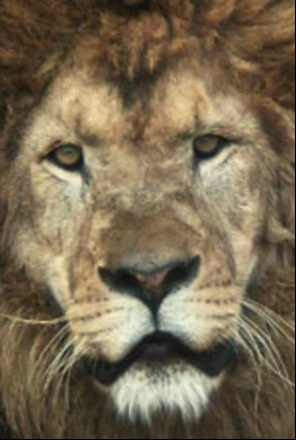
\includegraphics[width=0.17\textwidth]{../face_morphing/outputs/2/stage_8.jpg}
    }
    \subfigure[$\alpha = 7/9$]{
        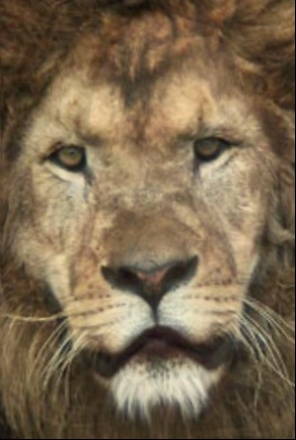
\includegraphics[width=0.17\textwidth]{../face_morphing/outputs/2/stage_7.jpg}
    }
    \subfigure[$\alpha = 6/9$]{
        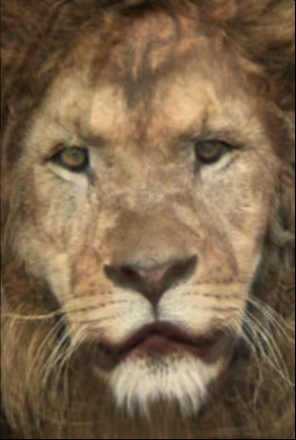
\includegraphics[width=0.17\textwidth]{../face_morphing/outputs/2/stage_6.jpg}
    }
    \subfigure[$\alpha = 5/9$]{
        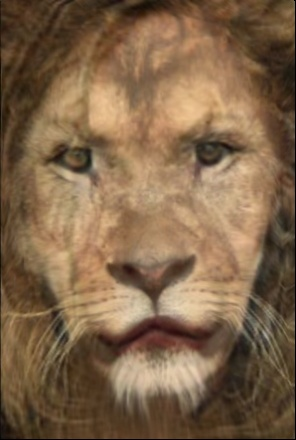
\includegraphics[width=0.17\textwidth]{../face_morphing/outputs/2/stage_5.jpg}
    }
    \caption{在不同的融合率$\alpha$下,第二组图片的融合效果}
    \label{fig:morph_result2}
\end{figure}

\section{View Morphing}

\subsection{方法}

实现思路主要参考了View Morphing的论文\cite{seitz1996view},考虑在不同视角下拍摄的原图和目标图,如果直接进行常规的morph,会使刚体发生扭曲和变形,不符合常理。为了维持刚体在变换中的刚性,论文提出了View Morphing框架,它主要分为三个步骤:首先将原图和目标图prewarp到同一平面上,然后进行常规的morph,最后将融合后的图像postwarp到所需视角。

常规的morph在Face Morphing任务中已经实现了,这里需要解决的问题主要是prewarp和postwarp的选取。对于prewarp,这里参考了论文的附录部分,通过求解基本矩阵$\mathbf{F}$,找到极点$\mathbf{e}_0$和$\mathbf{e}_1$,从而计算出原图和目标图的prewarp矩阵$\mathbf{H}_0$和$\mathbf{H}_1$,然后就可以将原图和目标图对齐到同一平面。

对于postwarp矩阵$\mathbf{H}_s$,按照论文对$\mathbf{H}_0$和$\mathbf{H}_1$加权平均的方法,得到的结果并不是太理想,因此这里选取一个Perspective Warp矩阵$\mathbf{H}_s$,使得融合后图像的四个角映射到最终图像的四个角,从而得到较为理想的效果。

理论上这三个步骤可以分步执行,但是实际上在prewarp或者morph的中间状态时,图像内容可能被边界遮挡,导致postwarp后图像残缺。因此,这里实现了完全端到端的变换,具体实现方法如下。

首先确定原图和目标图的prewarp矩阵$\mathbf{H}_0$和$\mathbf{H}_1$,将原图和目标图的对应点分别进行prewarp,沿用Face Morphing小节的符号,即得到$\{\mathbf{H}_0 \mathbf{p}_i\}_{i=1}^n$和$\{\mathbf{H}_1 \mathbf{q}_i\}_{i=1}^n$,同样求出中间状态,
\begin{equation}
    \mathbf{r}_i = (1-\alpha)\mathbf{H}_0 \mathbf{p}_i + \alpha \mathbf{H}_1 \mathbf{q}_i, \quad i = 1,2,\cdots,n
\end{equation}

对中间状态的特征点$\{\mathbf{r}_i\}_{i=1}^n$进行Delaunay三角剖分,对于某个Delaunay三角,记其从prewarp后的原图映射到中间状态的仿射变换为$\mathbf{A}$,然后用$\mathbf{H}_s$将中间状态的三角区域postwarp到最终状态,对于最终状态三角内一点$\mathbf{x}$,可以计算出其对应的原图坐标,即为$\mathbf{H}_0^{-1}\mathbf{A}^{-1}\mathbf{H}_s^{-1}\mathbf{x}$。这样就避免了引入中间状态,实现了端到端的变换。

\subsection{实现细节}

对于特征点的标注,这里采用\texttt{dlib}和人工结合的方式,其中\texttt{dlib}生成的面部特征点用于计算基本矩阵$\mathbf{F}$,并由此得到prewarp矩阵,其余的人工标注点连同\texttt{dlib}生成的点用于morph过程中的Delaunay三角剖分。

对于基本矩阵的求解,这里采用八点法,具体实现方法可参考维基百科\cite{eightpoint}。对于prewarp的选取,这里省略了论文中$\mathbf{H}_1$的平移和放缩矩阵$\textbf{T}$,原因是当$\mathbf{F}$的计算不准确时,$\textbf{T}$矩阵可能是奇异的。

\subsection{实验结果}

首先给出分步执行的结果,以第一组图片为例,当融合率$\alpha=0.5$时,prewarp后的原图和目标图,融合图像,以及postwarp后的融合图像如\Cref{fig:step},可以看出,prewarp导致原图的大量信息丢失,目标图被边界截断,导致morph后的图像出现裂缝,postwarp后出现残缺。

\begin{figure}[H]
    \centering
    \subfigure[Prewarped Source]{
        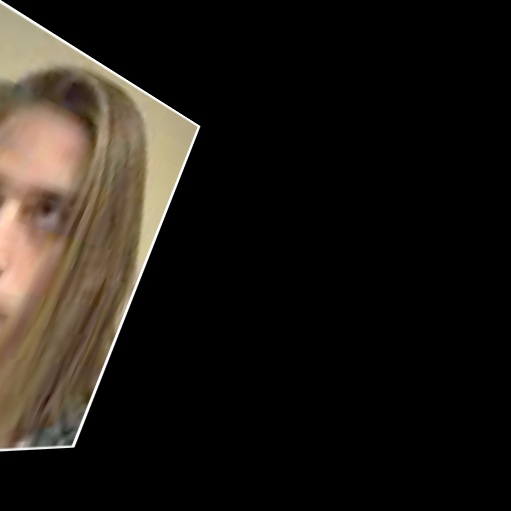
\includegraphics[height=0.23\textwidth]{../view_morphing/outputs/1/src_pre.jpg}
    }
    \subfigure[Prewarped Target]{
        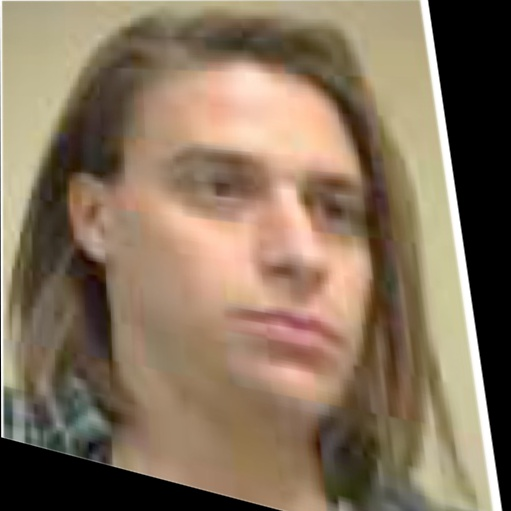
\includegraphics[height=0.23\textwidth]{../view_morphing/outputs/1/dst_pre.jpg}
    }
    \subfigure[Morphed]{
        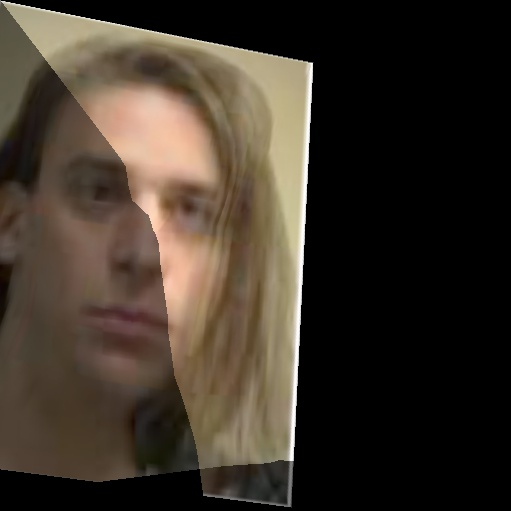
\includegraphics[height=0.23\textwidth]{../view_morphing/outputs/1/merged.jpg}
    }
    \subfigure[Postwarped]{
        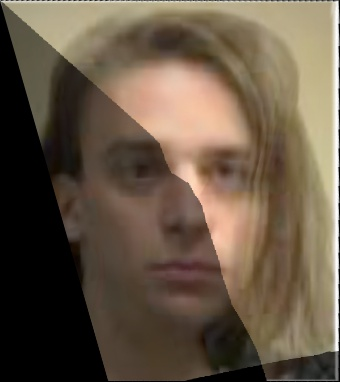
\includegraphics[height=0.23\textwidth]{../view_morphing/outputs/1/merged_post.jpg}
    }
    \caption{prewarp后的原图和目标图,postwarp前后的融合图像}
    \label{fig:step}
\end{figure}

为了弥补这一缺陷,这里实现了端到端的View Morphing,在给定的两组图片上,实验结果如\Cref{fig:view_result1}和\Cref{fig:view_result2},可以看到,生成的中间序列实现了视角的转换,且内容十分完整,没有出现残缺现象,仅有少量的artifact。

此外,这里还补充了两组图片,实验结果如\Cref{fig:view_result3}和\Cref{fig:view_result4},其中原图和目标图是通过镜面对称生成的,因此prewarp的计算结果更加准确,过渡也更自然。

\begin{figure}[H]
    \centering
    \subfigure[Source]{
        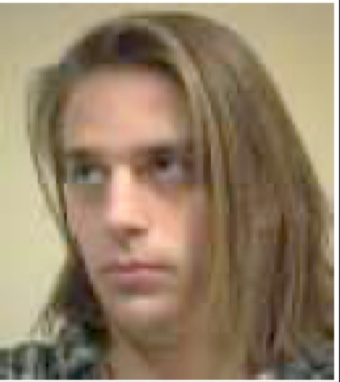
\includegraphics[width=0.17\textwidth]{../view_morphing/inputs/1/source.jpg}
    }
    \subfigure[$\alpha = 0.25$]{
        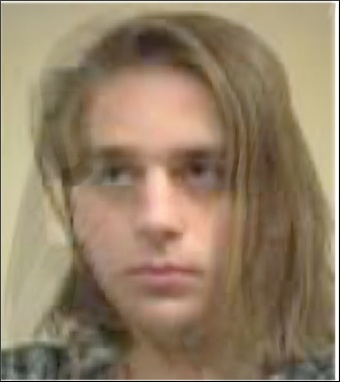
\includegraphics[width=0.17\textwidth]{../view_morphing/outputs/1/stage_1.jpg}
    }
    \subfigure[$\alpha = 0.50$]{
        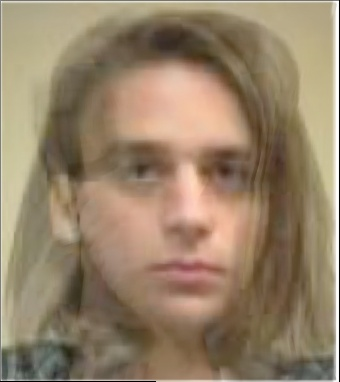
\includegraphics[width=0.17\textwidth]{../view_morphing/outputs/1/stage_2.jpg}
    }
    \subfigure[$\alpha = 0.75$]{
        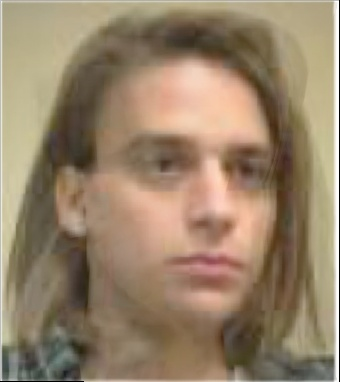
\includegraphics[width=0.17\textwidth]{../view_morphing/outputs/1/stage_3.jpg}
    }
    \subfigure[Target]{
        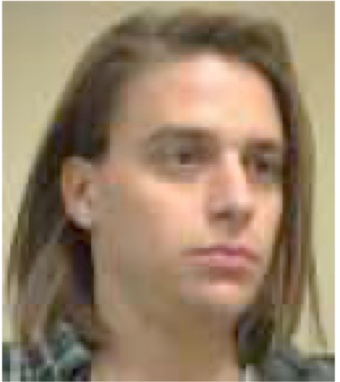
\includegraphics[width=0.17\textwidth]{../view_morphing/inputs/1/target.jpg}
    }
    \caption{在不同的融合率$\alpha$下,第一组图片的融合效果}
    \label{fig:view_result1}
\end{figure}

\begin{figure}[H]
    \centering
    \subfigure[Source]{
        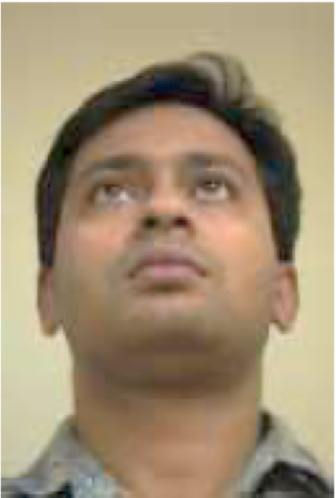
\includegraphics[width=0.17\textwidth]{../view_morphing/inputs/2/source.jpg}
    }
    \subfigure[$\alpha = 0.25$]{
        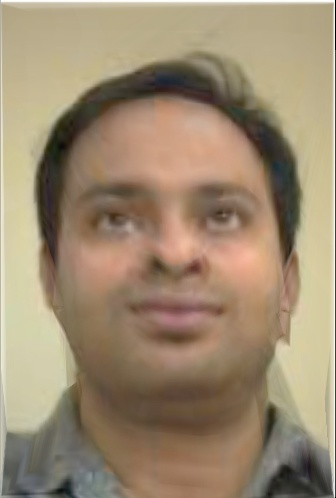
\includegraphics[width=0.17\textwidth]{../view_morphing/outputs/2/stage_1.jpg}
    }
    \subfigure[$\alpha = 0.50$]{
        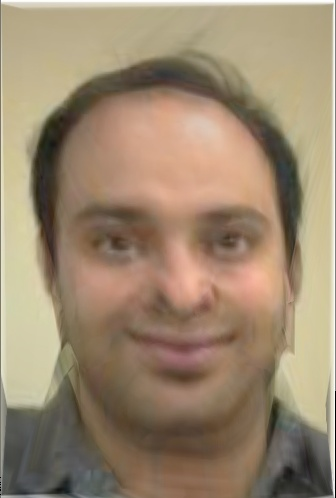
\includegraphics[width=0.17\textwidth]{../view_morphing/outputs/2/stage_2.jpg}
    }
    \subfigure[$\alpha = 0.75$]{
        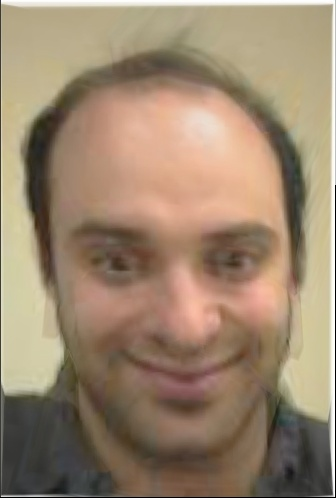
\includegraphics[width=0.17\textwidth]{../view_morphing/outputs/2/stage_3.jpg}
    }
    \subfigure[Target]{
        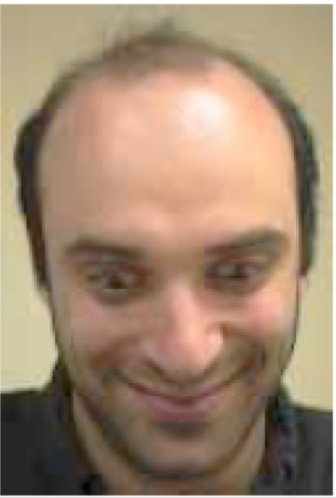
\includegraphics[width=0.17\textwidth]{../view_morphing/inputs/2/target.jpg}
    }
    \caption{在不同的融合率$\alpha$下,第二组图片的融合效果}
    \label{fig:view_result2}
\end{figure}

\begin{figure}[H]
    \centering
    \subfigure[Source]{
        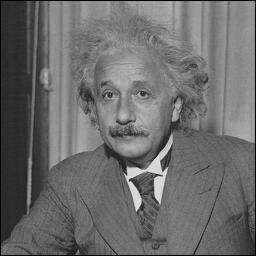
\includegraphics[width=0.17\textwidth]{../view_morphing/inputs/3/source.jpg}
    }
    \subfigure[$\alpha = 0.25$]{
        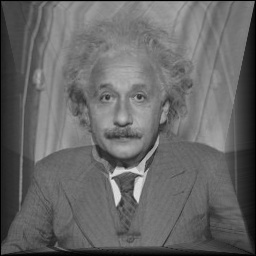
\includegraphics[width=0.17\textwidth]{../view_morphing/outputs/3/stage_1.jpg}
    }
    \subfigure[$\alpha = 0.50$]{
        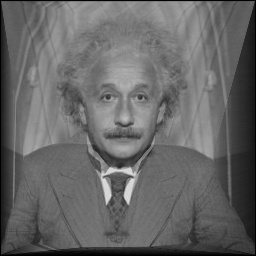
\includegraphics[width=0.17\textwidth]{../view_morphing/outputs/3/stage_2.jpg}
    }
    \subfigure[$\alpha = 0.75$]{
        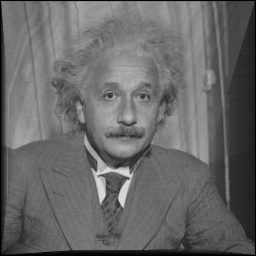
\includegraphics[width=0.17\textwidth]{../view_morphing/outputs/3/stage_3.jpg}
    }
    \subfigure[Target]{
        \includegraphics[width=0.17\textwidth]{../view_morphing/inputs/3/target.jpg}
    }
    \caption{在不同的融合率$\alpha$下,第三组图片的融合效果}
    \label{fig:view_result3}
\end{figure}

\begin{figure}[H]
    \centering
    \subfigure[Source]{
        \includegraphics[width=0.17\textwidth]{../view_morphing/inputs/4/source.jpg}
    }
    \subfigure[$\alpha = 0.25$]{
        \includegraphics[width=0.17\textwidth]{../view_morphing/outputs/4/stage_1.jpg}
    }
    \subfigure[$\alpha = 0.50$]{
        \includegraphics[width=0.17\textwidth]{../view_morphing/outputs/4/stage_2.jpg}
    }
    \subfigure[$\alpha = 0.75$]{
        \includegraphics[width=0.17\textwidth]{../view_morphing/outputs/4/stage_3.jpg}
    }
    \subfigure[Target]{
        \includegraphics[width=0.17\textwidth]{../view_morphing/inputs/4/target.jpg}
    }
    \caption{在不同的融合率$\alpha$下,第四组图片的融合效果}
    \label{fig:view_result4}
\end{figure}

\bibliographystyle{abbrv}
\bibliography{report}

\end{document}